\section*{\underline{Aufgabe 1}}

\subsection*{a)}

Der geringste mittlere quadratische Fehler ist bei einem Radius von 0.45 aufgetretten, cdaher wählen wir für den optimalen Radius diesen Wert.

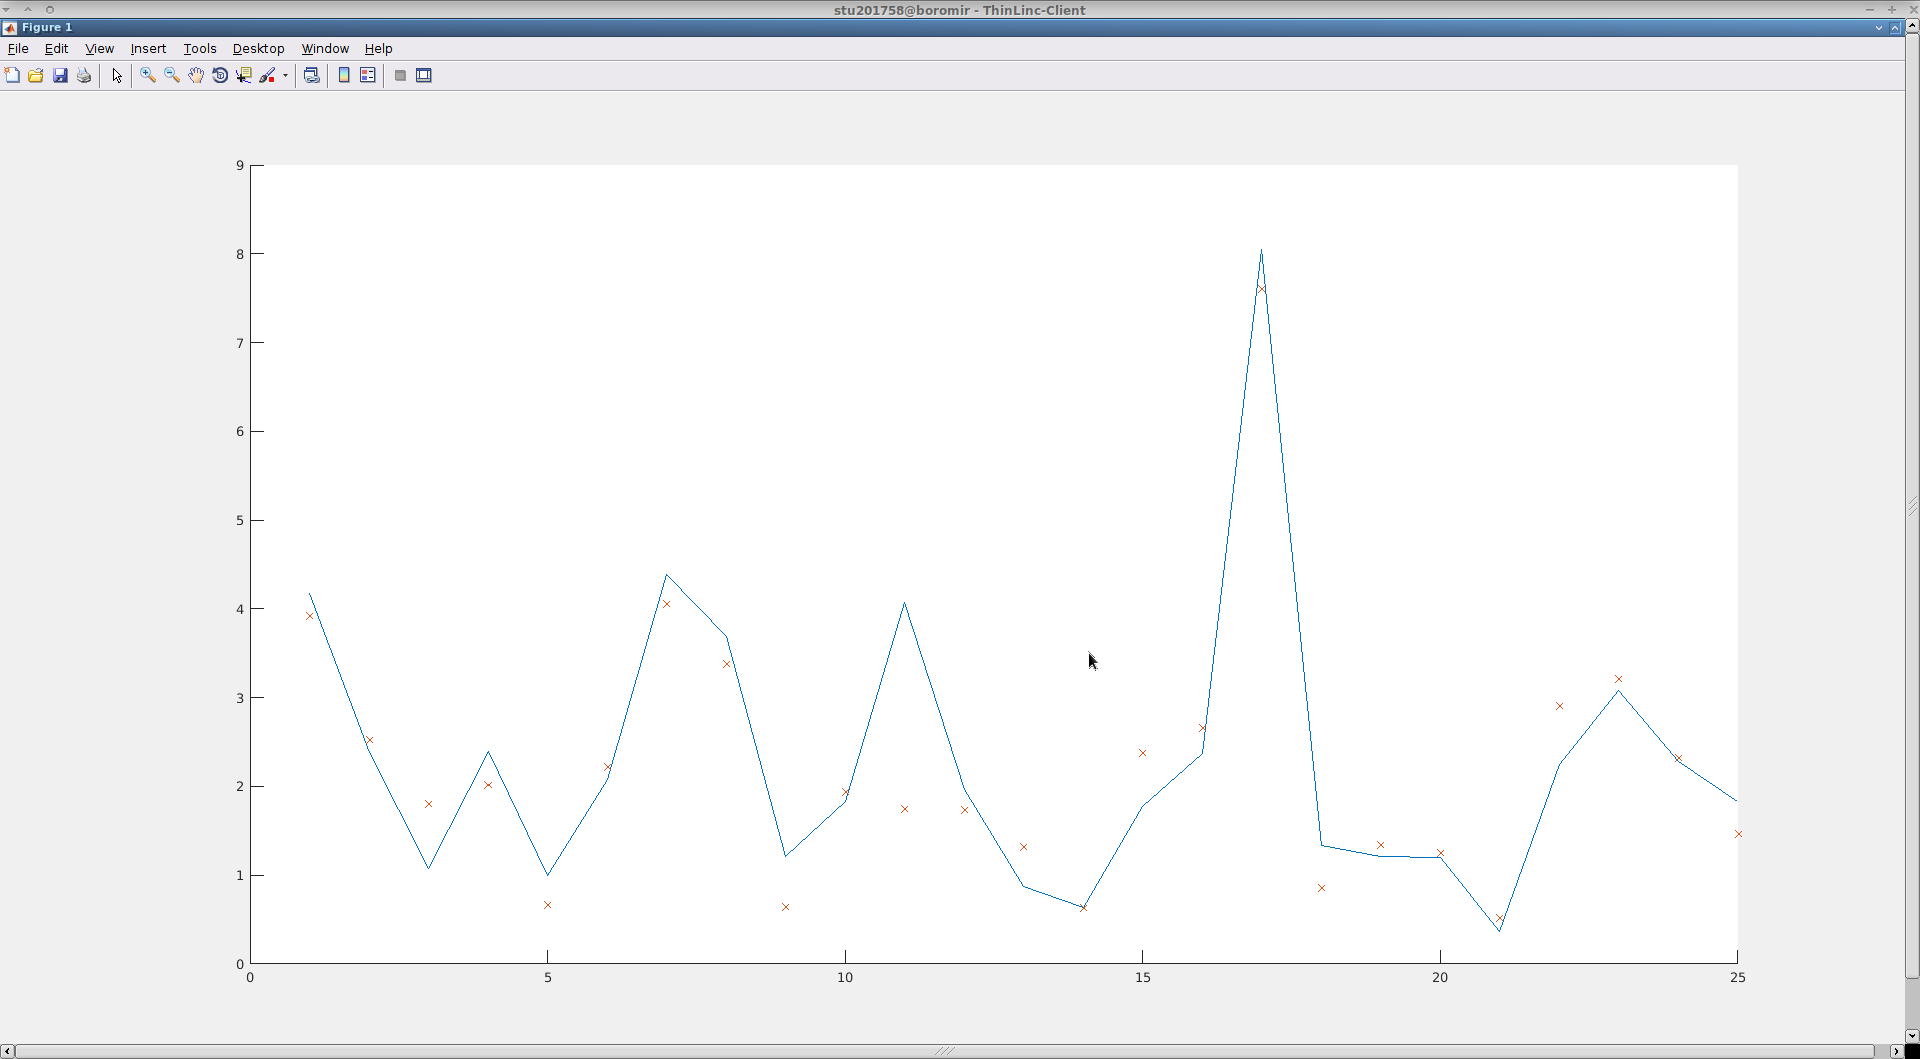
\includegraphics[width=\textwidth]{part/S9-A1a-Plot}

Die Linie Bezeichnet die vom Modell berechneten Werte, die Kreuze bezeichnen die Realdatan von chkdatout.

\subsection*{b)}

Im Model finden sich vier Regeln.

Die Paramater für den Konklusionsteil sind:

\begin{verbatim}
out1cluster1:  [ -0.7375 -0.0442  0.2956 -0.09886 0.913   3.368  ]

out1cluster2:  [ -0.2641 -0.2485  1.404   0.0162  1.457   0.3862 ]

out1cluster3:  [ -2.277  -1.502   6.061   0.07259 0.4756 -0.1332 ]

out1cluster4:  [  3.02   -1.324  -3.421   0.05444 0.8892 -0.6473 ]
\end{verbatim}

\clearpage

\subsection*{c)}

Mit subclust wurden vier Cluster ermittelt, mit den Zenter-Koortinaten:

\begin{verbatim}
Cluster 1   [ 1.4460    1.5070    0.6570    0.7060   15.7350    0.6360 ]
Cluster 2   [ 2.3850    3.1160    1.1930    1.4870   19.7330    0.6030 ]
Cluster 3   [ 0.7680    0.0440    0.0240    0.0210    9.3400    0.8500 ]
Cluster 4   [ 3.2530    1.7270    0.6900    1.2320   30.5730    1.3970 ]
\end{verbatim}